\chapter{Vooruitblik}
\label{ch:vooruitblik}

De markt voor cryptocurrencies is nog altijd zeer fluctuerend en grotendeels ongereguleerd. Om deze reden is het nog steeds speculatief om in deze markt te investeren. Er is veel discussie over hoe we blockchain en cryptocurrencies kunnen implementeren, maar ondertussen wordt er wel keihard aan de weg getimmerd. Grote technologische en wetenschappelijke doorbraken werden nooit vanaf dag {\'e}{\'e}n alleen maar lovend ontvangen.\bigskip



\section*{De FinTech-sector}
De cryptocurrency-markt biedt onge{\"e}venaard potentieel. De mogelijkheden voor explosieve groei van investeringen op de lange termijn zijn aanzienlijk. Aangezien vrijwel alle cryptocurrencies nog in de kinderschoenen staan, is het verre van zeker of deze allemaal succesvol zullen zijn. Het is zeer aannemelijk dat enkele van deze projecten hun marktpositie de komende maanden en jaren verder zullen consolideren, maar niemand kan met 100\% zekerheid voorspellen welke. Daarnaast starten er bijna dagelijks vele andere cryptocurrency-projecten. Het is een snel-groeiend ecosysteem van start-ups die de ineffici{\"e}nte systemen binnen de financi{\"e}le sector aanvliegen.

  \bigskip
    \begin{quotation}
          \textit{\say{Voor een transitie kom je te vroeg of te laat, je bent nooit op tijd.}}
          \begin{flushright}
            \small{--- \textbf{Derk Loorbach}}
          \end{flushright}
    \end{quotation}


\section*{Transitie}
Logisch gevolg van zo'n snel groeiende en evoluerende nieuwe sector is dan ook een tekort aan bijvoorbeeld programmeurs en software-ingenieurs. Update jouw kennis en wees je bewust van deze transitie, want binnen de financieel technologische (fintech) sector zijn grote en steeds snellere veranderingen gaande. Vrijwel iedereen kan meedoen aan deze transitie, bijvoorbeeld door via internet cursussen te volgen en nieuwe vaardigheden te leren die jouw carri{\`e}re een enorme boost of wending kunnen geven.  

\section*{Blockchain-revolutie}
Het succes van blockchain en distributed ledger technologie staat eigenlijk al vast, omdat deze technologie niet afhankelijk is van cryptocurrency. Cryptocurrency is slechts een functionaliteit van de blockchain; er kan namelijk ook gebruik worden gemaakt van blockchain zonder cryptocurrency - de mogelijkheden zijn eindeloos. 

\section*{Internet of Value}
Wij zijn, samen met vele anderen, van mening dat distributed ledger technologie een integraal onderdeel zal vormen van onze toekomstige informatie-infrastructuur. Deze ontwikkelingen vormen een nieuwe laag op het internet, ontwikkelingen die nieuwe eigenschappen cre\"eren. De uitdagingen liggen vooral in de adoptie en implementatie. Hoe moet omgegaan worden met deze technologie door verschillende partijen? Enerzijds kan de technologie gebruikt worden om meer controle uit te oefenen, anderzijds biedt open blockchain technologie fantastische nieuwe eigenschappen zoals volledige transparantie, eerlijkheid en totale onveranderlijkheid. Het biedt bovendien het individu de mogelijkheid weer zeggenschap te krijgen over financi{\"e}le middelen. Overheden en regulerende instanties zullen alle zeilen bij moeten zetten om de adoptie van blockchain en cryptocurrencies in goede banen te leiden, zonder deze innovatie in de kiem te smoren. 


\newpage 

\section*{Waarom nu een goed moment is}
Er is vaak een (ernstige) crisis nodig om de nodige veranderingen teweeg te brengen. De huidige pandemie en de impact ervan op onze geglobaliseerde samenleving zijn enorm  en zullen een versnelde en onge{\"e}venaarde financi{\"e}le crisis teweegbrengen. Nu meer dan ooit is het moment aangebroken om ons te verdiepen in vernieuwende financi{\"e}le technologie{\"e}n.
In de volgende {\fontseries{extrabold}\selectfont cryptomanual}; \say{{\fontseries{medium}\selectfont enter cryptocurrencies}} gaan wij verder in op onder andere de volgende onderwerpen:

\begin{enumerate}[label=(\alph*)]
  \setlength\itemsep{0em}
    \item Open en Gedecentraliseerde Finance.
    \item Wat zijn geld, goud en valuta?
    \item De geschiedenis en toekomst van geld.
    \item Digitalisatie 2.0. - \say{The Internet of Value}
    \item De start van een nieuw tijdperk - \say{Ice Age of Cryptocurrencies}.
\end{enumerate}



\begin{figure}
\centering
    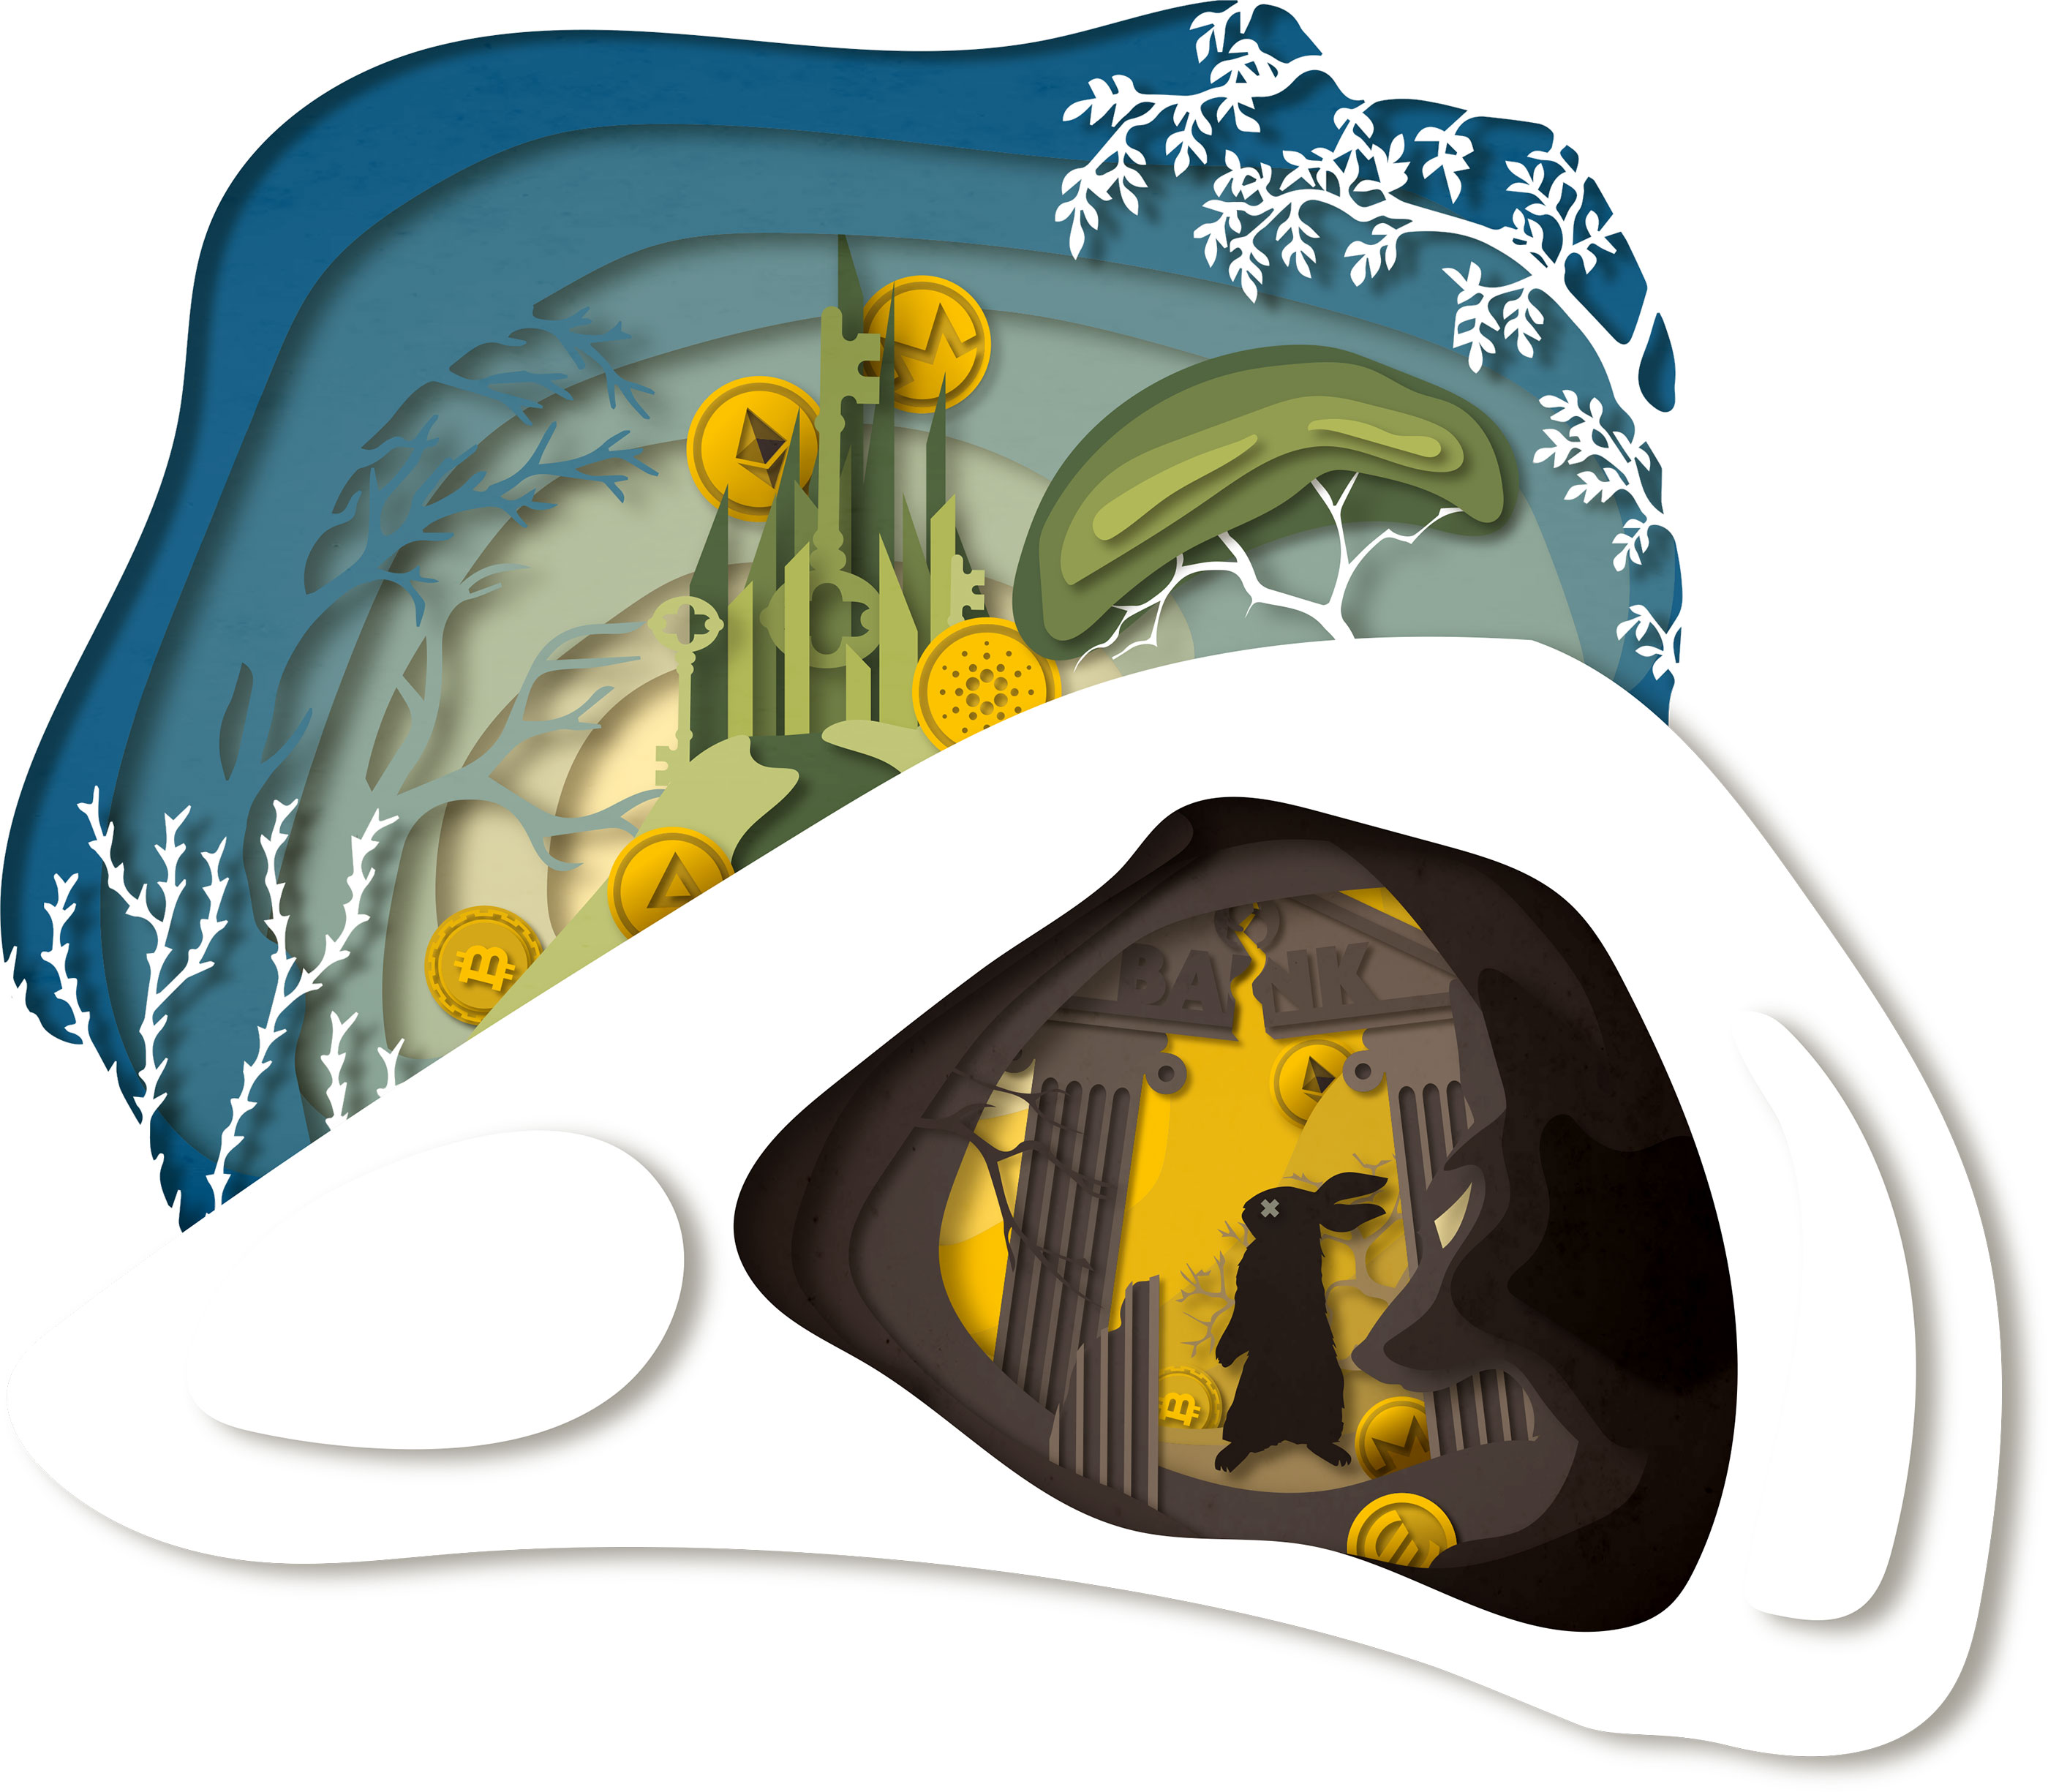
\includegraphics[width=\textwidth]{illustrations/resized_CRYPTO_KEY_1_PART_2.jpg}
\end{figure}


